%! TEX root = part2.tex
% the main TeX file which is intended to compile, :VimtexReload after adjustment
% :h vimtex-tex-root
\documentclass[../main.tex]{subfiles}
%ensure the class of docs

\begin{document}

\begin{frame}[t,mycolor=digiPH_gray,mytitle=standard,dark]

	\includegraphics<1-2>[width=.75\textwidth]{batukp}

	\only<2>{\boldblue{batu Kapur} }


	\includegraphics<3-4>[width=.75\textwidth]{bc1d-S}

	\only<4>{\boldred{granit} }

	\includegraphics<5-6>[width=.75\textwidth]{84-vhBp}

	\only<6>{\boldblue{Batu Pasir} }

\end{frame}



\begin{frame}[label=current,t,mycolor=digiPH_gray,mytitle=standard,light]
	\frametitle{Batu sebagai bahan bangunan}
	\framesubtitle{jenis tanah liat}

	\boldblue{Tanah Liat Primer}

	adalah tanah liat yang dihasilkan dari pelapukan batuan felspar tanpa berpindah tempat.  Jenis tanah liat primer: kaolin, bentonit, feldspatik, kuarsa, dan dolomit. Biasanya terdapat di  tempat-tempat yang tinggi.

	\textbf{Karakteristik:}

	\begin{itemize}
		\item Berwarna putih atau putih kusam;
		\item Butirannya kasar;
		\item Tidak plastis;
		\item Daya lebur tinggi;
		\item Daya susut kecil;
		\item Tahan terhadap api.
	\end{itemize}

\end{frame}


\begin{frame}[t,mybg=73-Ylnq,mytitle=standard,light]
	\frametitle{tanah lait sekunder}

	\txt{digiPH_white}{digiPH_black}{adalah tanah liat yang dihasilkan dari pelapukan batuan dengan berpindah tempat. Endapan  tanah liat ini terdapat di dataran rendah seperti sungai dan rawa. Tanah liat ini banyak  digunakan untuk keperluan konstruksi.}

	\txt{digiPH_white}{digiPH_black}{\textbf{Karakteristik:  }
		\begin{itemize}
			\item Berwarna krem/abu-abu/coklat/merah jambu/kuning, kuning  muda, kuning kecoklatan, kemerahan, kehitaman;
			\item Butirannya halus;
			\item Plastis;
			\item Suhu bakar antara 9.000 - 14.000 derajat celcius;
			\item Daya susut besar.
		\end{itemize}}

	\footnotesize Hasil olahan tanah liat (disebut juga lempung) yang sering digunakan dalam konstruksi bangunan adalah  batu bata, genteng, dan ubin.

\end{frame}

\begin{frame}[t,mybg=73-Ylnq,mytitle=standard,light]
	\frametitle{Batu Bata}

	\txt{digiPH_ocean}{digiPH_white}{Batu-bata sering disebut dengan bata merah. Berasal dari material tanah liat yang dicetak,  dikeringkan di bawah sinar matahari, atau dibakar dalam tungku pembakaran. Batu bata umumnya  digunakan sebagai bahan bangunan untuk konstruksi dinding.}

	\only<2>{
		\txt{digiPH_ocean}{digiPH_white}{\textbf{Karakteristik:}
			\begin{itemize}
				\item Sisi-sisi batu bata harus datar;
				\item Bersudut siku-siku dan tajam;
				\item Tidak mudah hancur atau patah;
				\item Permukaannya rata, kasar, dan tidak retak;
				\item Warna merahnya merata;
				\item Berbunyi nyaring bila diketuk.
			\end{itemize}}
	}

	\only<3>{
		\txt{digiPH_white}{digiPH_black}{\begin{tabular}[c]{l|l|l|l}
				Ukuran   &  Jenis besar(mm)  &  Jenis kecil(mm)  &  toleransi(mm)  \\
				\hline
				Panjang  &  240              &  230              &  selisi maks.10  \\
				Lebar    &  115              &  110              &  selisi maks.5  \\
				Tinggi   &  52               &  50               &  selisi maks.4  \\
				\hline
			\end{tabular}}
	}

\end{frame}


\begin{frame}[t,mytitle=standard,light]
	\frametitle{Batu Bata}

	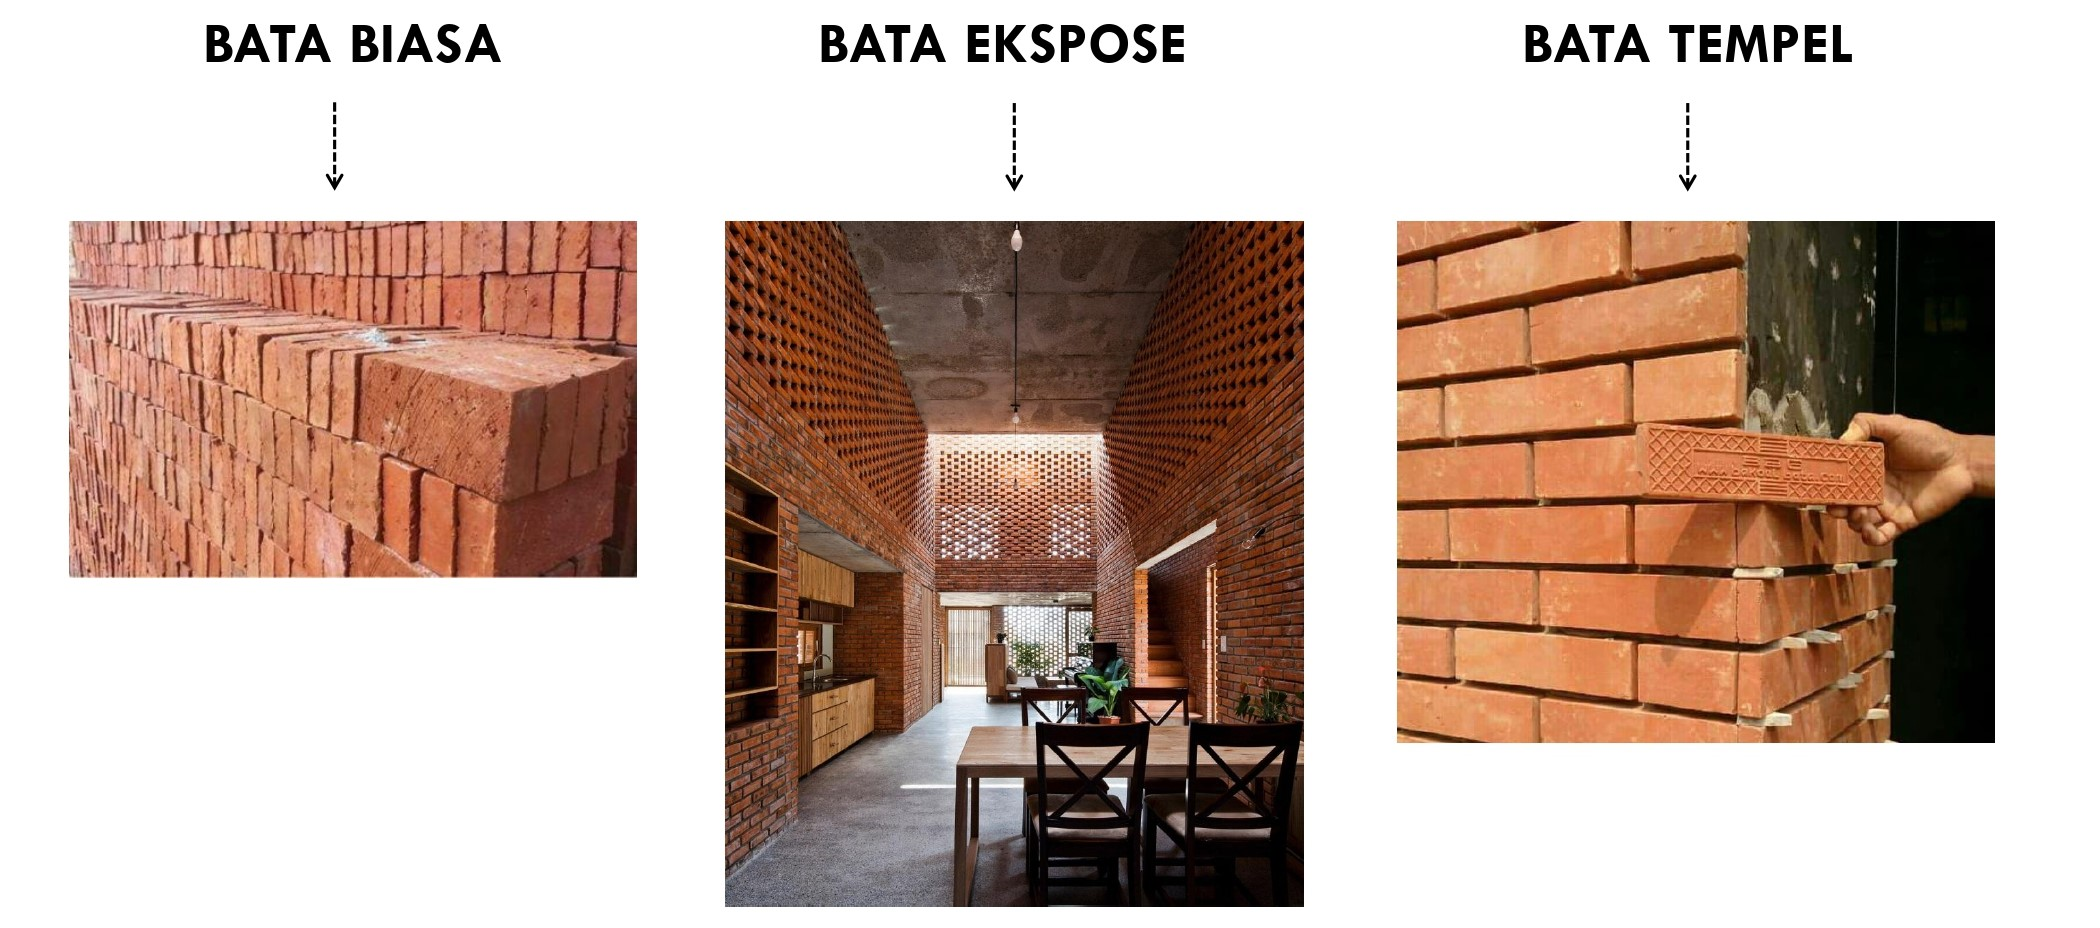
\includegraphics[width=.9\textwidth]{40-MGZS}
	\begin{columns}
		\begin{column}{0.3\textwidth}
			\only<2->{\boldblue{Struktural} }
		\end{column}
		\begin{column}{0.7\textwidth}
			\only<3->{\boldred{Arsitektural} }
		\end{column}
	\end{columns}
\end{frame}

\begin{frame}[t,mytitle=standard,light]

	\frametitle{Batu Bata}

	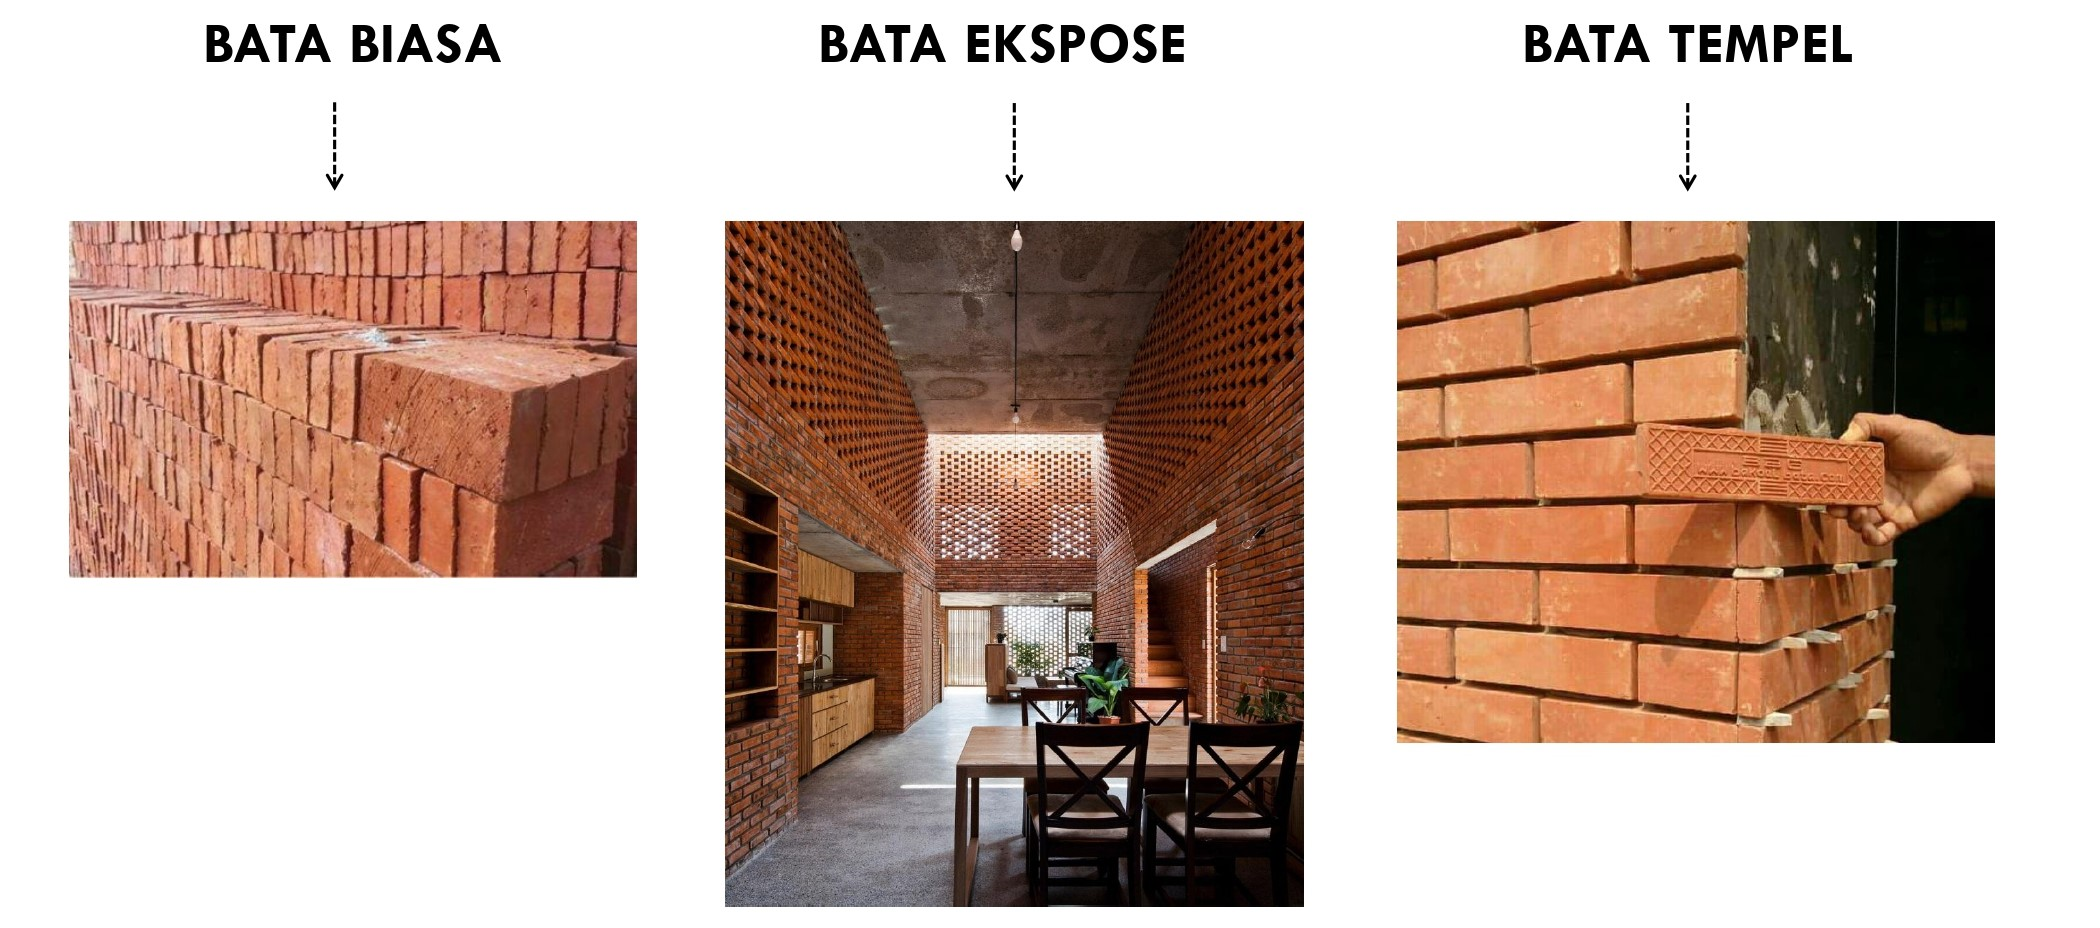
\includegraphics[width=.9\textwidth]{40-MGZS}
	\only<2>{
		\txt{digiPH_white}{digiPH_black}{\footnotesize \boldblue{Struktural} \\ Bata serba guna untuk penggunaan  umum  dan  tidak  diperlakukan  secara khusus untuk warna dan  tekstur, biasa disebut sebagai bata  bangunan.}
	}
	\only<3>{
		\txt{digiPH_white}{digiPH_black}{\footnotesize
			\boldblue{Arsitektural} \\
			Bata dari tanah liat khusus yang digunakan pada permukaan  dinding, sering diperlakukan secara khusus untuk menghasilkan  warna-warna tertentu, dan juga tekstur permukaan yang  diinginkan }
	}
\end{frame}

\begin{frame}[t,mybg=73-Ylnq,mytitle=standard,light]
	\frametitle{Bata Biasa}
	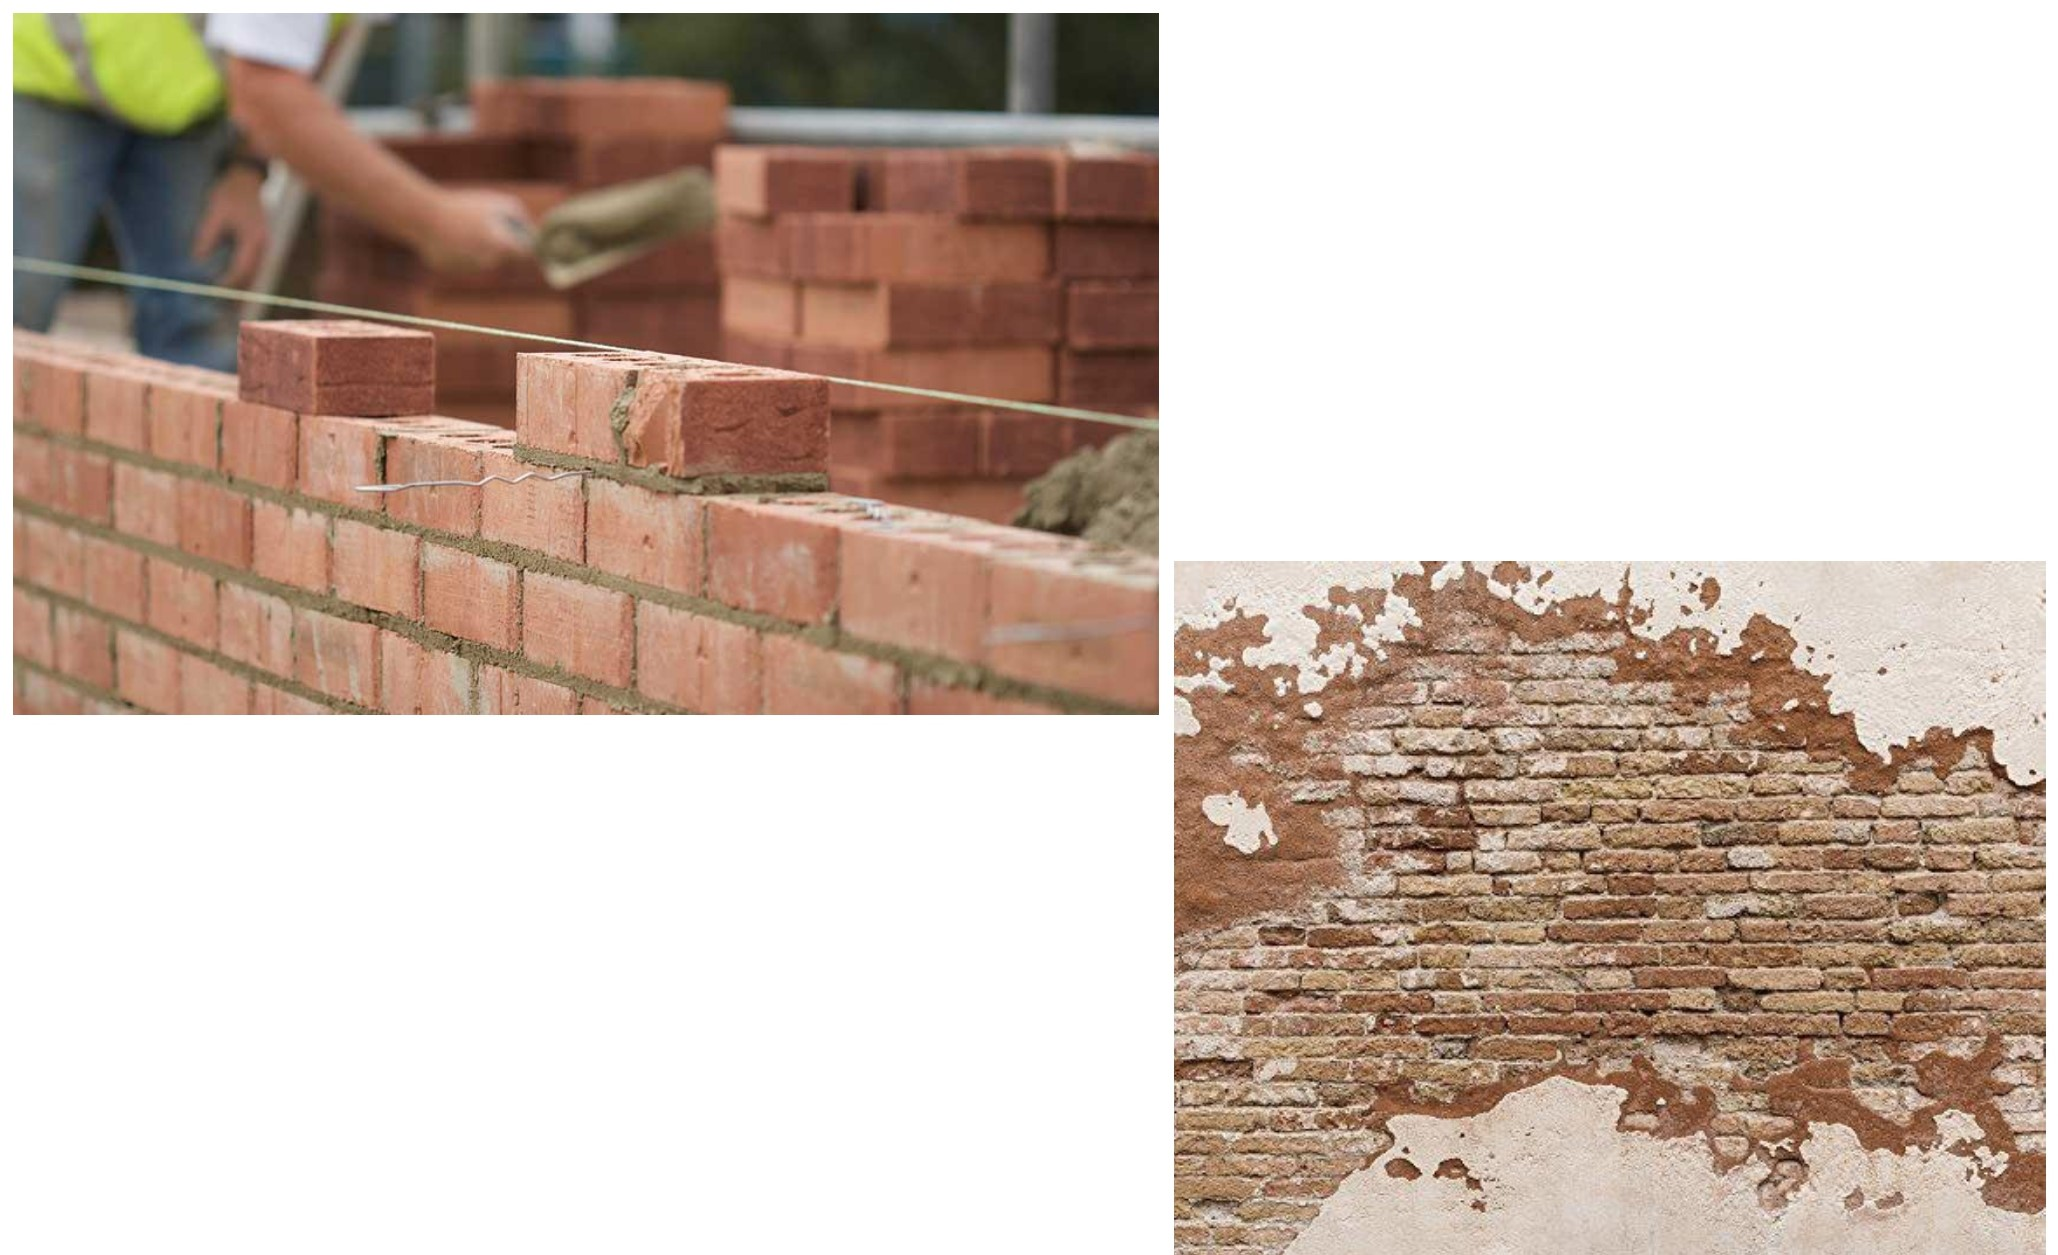
\includegraphics[width=.9\textwidth]{2}
\end{frame}

\begin{frame}[t,mybg=73-Ylnq,mytitle=standard,light]
	\frametitle{Bata Ekspos}
	\only<1->{\limg{14-kTo9}}
	\only<2->{\rimg{32-BgKO}}
\end{frame}


\begin{frame}[t,mybg=57-nqQU,mytitle=standard,dark]
	\frametitle{Bata Ekspos}
	\only<1->{\limg{91-P90o}}
	\only<2->{\rimg{67-0wGe}}
\end{frame}


\begin{frame}[t,mycolor=digiPH_red,mytitle=standard,dark]
	\frametitle{Batu bata}
	\begin{bgblock}{0mm}{0mm}%130x95
		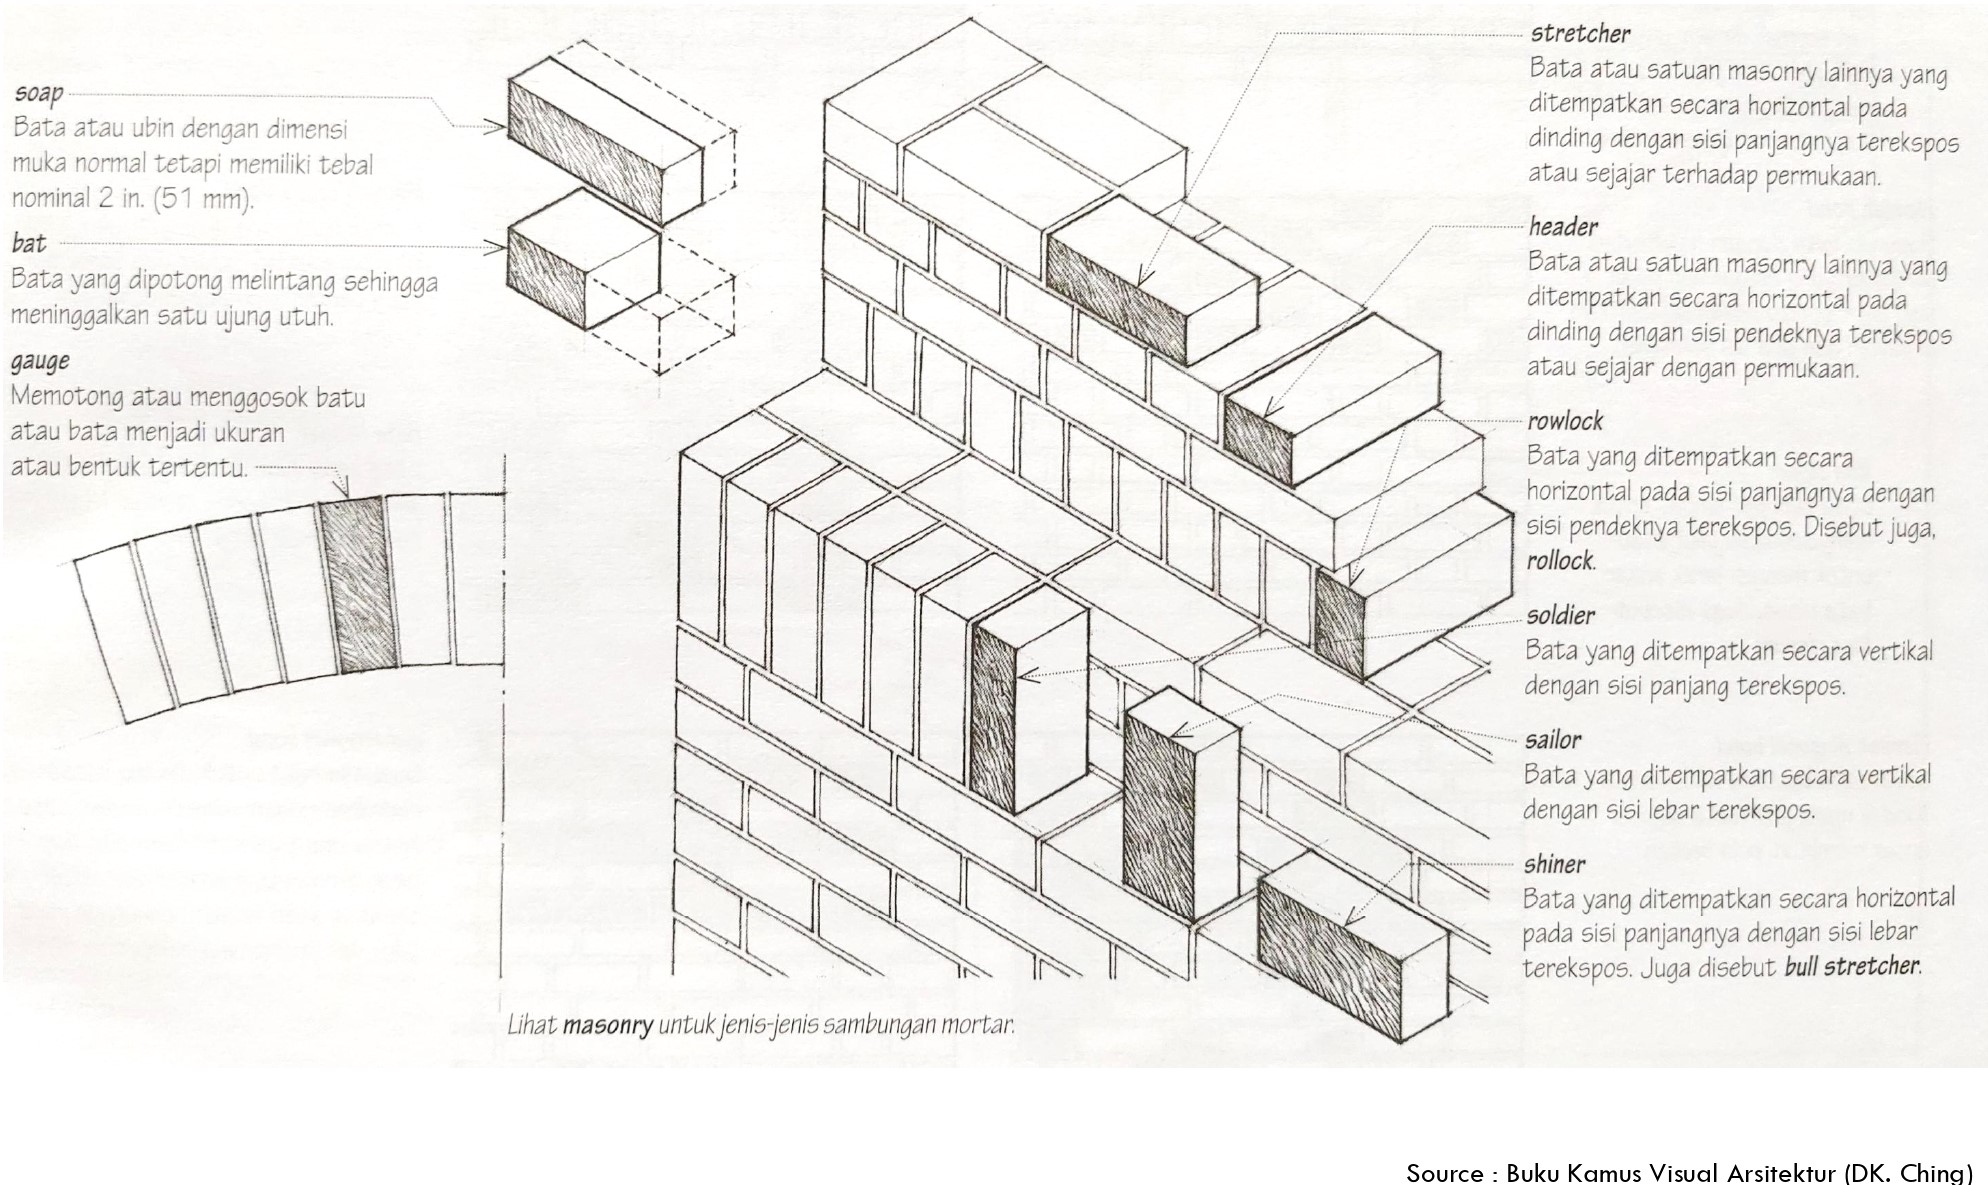
\includegraphics[width=\paperwidth]{32-W2Tu}
	\end{bgblock}
\end{frame}

\begin{frame}[t,mytitle=standard,light]
	\frametitle{Batu bata}
	\framesubtitle{Teknik dan Istilah penyusunan Bata}
	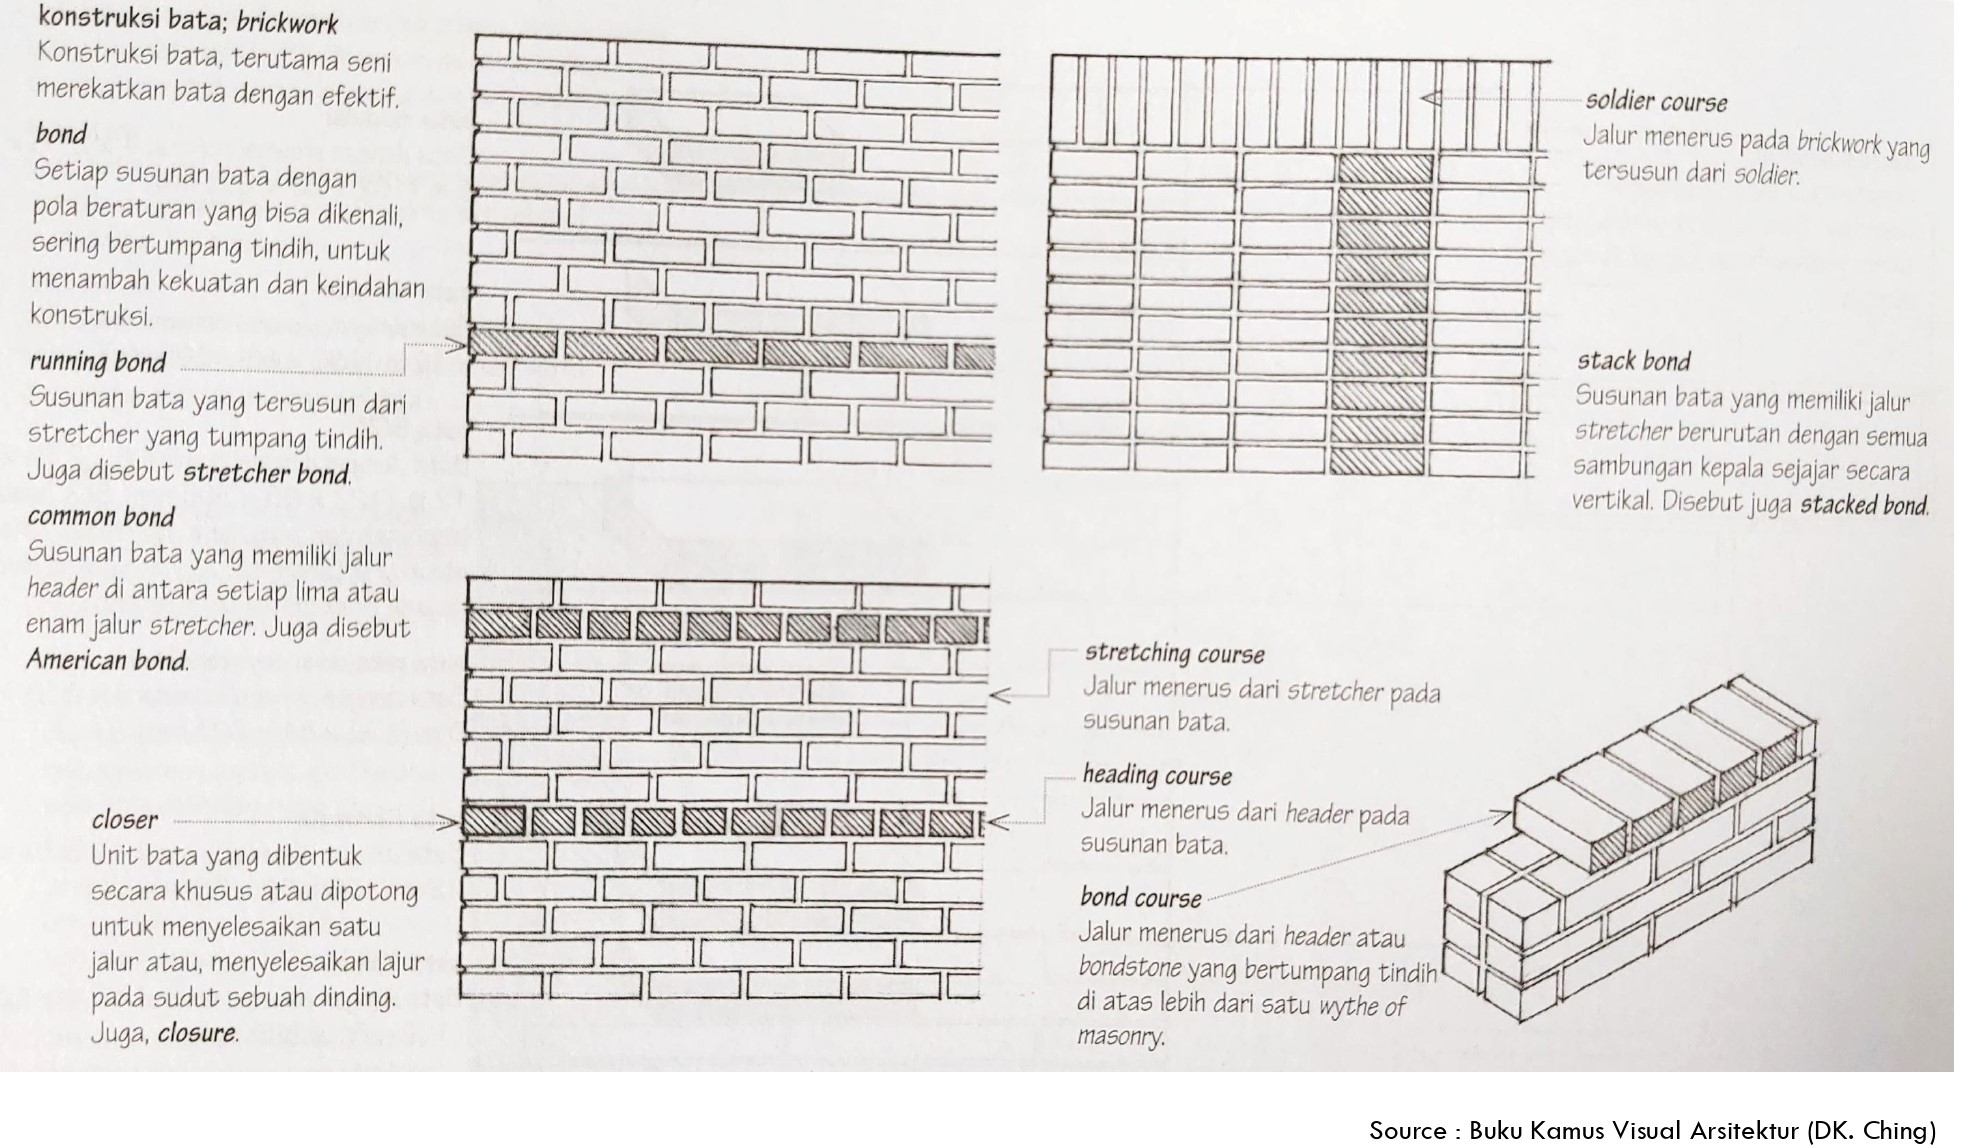
\includegraphics[width=.9\textwidth]{45-nWbd}
\end{frame}

\begin{frame}[t,mytitle=standard,light]
	\frametitle{Teknik dan Istilah penyusunan Bata}

	\only<1->{\limg{80-PNKE}}
	\only<2->{\rimg{70-NTRB}}
\end{frame}

\begin{frame}[t,mytitle=center,light]
	\frametitle{Teknik dan Istilah penyusunan Bata}
	\only<1->{\limg{35-hFW0}}
	\only<2->{\rimg{37-pxuy}}

	{\footnotesize sumber : Buku Kamus Visual Arsitektur(DK. Ching}
\end{frame}


\begin{frame}[t,mybg=57-nqQU,mytitle=standard,light]
	\only<1->{\limg{dkching}}
	\only<2->{\rtxt{digiPH_red}{digiPH_white}{Buku \textbf{Kamus Visual Arsitektur}
			\\
			\\
			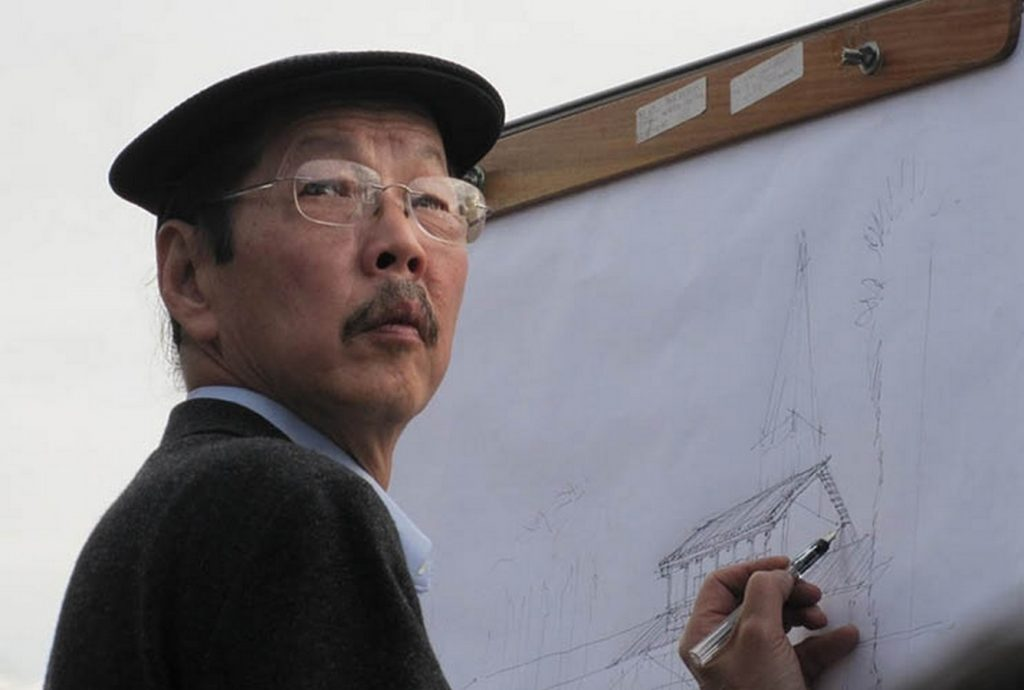
\includegraphics[width=.9\textwidth]{dkchingg}
		}}
\end{frame}


\begin{frame}[t,mycolor=digiPH_leaf,mytitle=standard,dark]
	\frametitle{Tugas}
	\txt{digiPH_gray}{digiPH_white}{\begin{itemize}
			\small
			\item Tiap mahasiswa \boldred{membuat sebuah resume/rangkuman}  dari gabungan materi kuliah 2 \& 3 (Pertemuan 2 \& 3) yakni sifat, jenis-jenis batuan yang digunakan pada bahan bangunan.
			\item \textit{Gunakan bahasa dari pemahaman anda sendiri}  setelah membaca materi.
			\item Resume/rangkuman dibuat dalam ukuran kertas HVS A4, maksimal 2 halaman.
			\item Resume/rangkuman dibuat secara digital (boleh diketik), atau manual (tulis tangan). Tambahan berupa sketsa-sketsa (warna) akan menjadi nilai tambah.
			\item Jangan lupa beri keterangan NAMA \& NIM pada bagian atas (kiri/kanan) halaman pertama.
			\item Bagi yang membuat tugas secara manual, harap untuk difoto yang jelas. Format file tugas boleh dalam .jpeg ataupun .pdf, dengan ukuran file tidak lebih dari 5mb.
			      % \item Waktu pengumpulan sampai satu minggu kedepan (Jumat 16 Oktober 2020), dikumpulkan dengan cara upload file tugas melalui SCE.
		\end{itemize}}

\end{frame}

\bibliographystyle{apalike}
\bibliography{../filename.bib} % required for citecompletion, not work in mainfile
\end{document}

